%Chapter 2 is a primer on parallel algorithms and specifically CUDA design principles
%Also describes the CPU/GPU Architecture at a high level
\chapter{Parallel Programming Paradigms}
\label{chap:parallelprogramming}
This chapter will provide and introduction to the fundamentals parallel programming. The remaining chapters will assume a working knowledge of parallel algorithms, GPU architecture, and CUDA optimization techniques.
\section{Principles of Parallel Programming}
As the physical limits of transistor size are being reached, the trend in computing has been away from making processors faster and towards parallel processing. The introduction of General Purpose Graphics Processing Units have made data parallel algorithms a very attractive approach to accelerating computationally intensive tasks. However, migrating from sequential computing to parallel platforms is not always simple or even wise. The following are some principles to keep in mind when considering using GPU acceleration.\par
\paragraph{Keep data parallel} 
Parallel computing is best suited to performing simple operations on large numbers of independent data elements, such as n-body simulations and per-pixel image processing operations. Aside from these trivial cases, adapting sequential algorithms to a GPU architecture efficiently can be challenging. Not all loops are easily parallelizable.
\paragraph{Memory is a bottleneck}
Computing with thousands of cores in a GPU makes memory I/O into a major bottleneck. Usually the data transfer to and from the parallel device will take much longer than the actual compute time. Be extremely conscious of memory usage and access patterns.
\paragraph{Minimize code divergence}
On most architectures, parallel code runs in batches for increased efficiency. If the code is full of if/then/else statements, the divergent execution paths can dramatically impact performance.
\paragraph{Avoid sequential operations and synchronization}
Atomic operations that must be performed in order or synchronizations between concurrent threads of execution can be very slow. The more the threads can be independent of each other, the more efficiently the hardware will be able to execute them in parallel.
\paragraph{Be mindful of the hardware}
When writing performance critical code, understanding the underlying architecture can be a big help. Understanding how the code will actually be distributed and executed across multiple processors will make optimization much easier.

\section{Parallel Algorithm Building Blocks}
Just as there are fundamental building blocks of sequential computing like search, recursion, and iteration, many parallel algorithms make use of primitive operations like reduce, scan, and stream compact.
\subsection{Reduction}
Reduction is any operation on an array of elements that computes a single result. Common examples include sums, average, min, max, and product. In sequential terms, implementing reduction is very simple. Using sum as an example, algorithm~\ref{alg:sequentialsum} shows how this might be implemented.\\
\begin{algorithm}[!htpb]
\label{alg:sequentialsum}
 \singlespacing
 \KwData{n element array X}
 \KwResult{sum of elements in X}
 i = 0\;
 sum = 0\;
 \While{i $<$ n}{
  sum += X[i]\;
  i++\;
 }
 \caption{Sequential Sum}
\end{algorithm}

Notice that in the sequential algorithm, the accumulator's value at each iteration depends on the value in the previous iteration. To perform a parallel sum, the associative property of the operator can be exploited to break group the operation into a structured set of binary operations that can be performed in parallel (Figure~\ref{fig:reductionsum}).
\begin{figure}[ht]
    \centering
    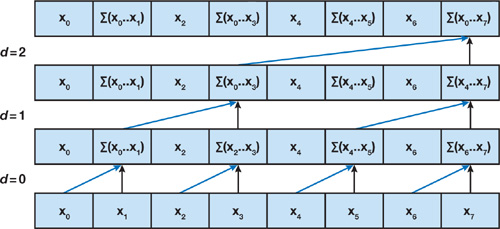
\includegraphics[width=\textwidth]{ReductionSum.jpg}
    \caption{Parallel Reduction. Reproduced from\cite{nguyen2007gpu}}
    \label{fig:reductionsum}
\end{figure}

This parallel reduction method will work for any associative binary operator.

\subsection{Scan}
The scan operation is similar to a performing a cumulative sum operation on an array. There are two forms of scan: exclusive and inclusive. Usually the term scan refers to an exclusive scan.\par
Given an associative binary operator $\oplus$ with identity value $I$ and an array of $n$ items $[a_0, a_1, \ldots a_{n-1}]$, an exclusive scan returns the array: $$[I, a_0, (a_0 \oplus a_1), (a_0 \oplus a_1 \oplus a_2),\ldots, (a_0 \oplus a_1 \oplus \ldots \oplus a_{n-2})]$$ An inclusive scan returns the shifted result:  $$[a_0, (a_0 \oplus a_1), (a_0 \oplus a_1 \oplus a_2),\ldots, (a_0 \oplus a_1 \oplus \ldots \oplus a_{n-1})]$$ The sequential implementation of a sum scan is trivial and outlined in Algorithm~\ref{alg:sumscan}.

\begin{algorithm}[!htpb]
\label{alg:sumscan}
 \singlespacing
 \KwData{n element array X}
 \KwResult{array Y contains exclusive scan of X}
 i = 1\;
 Y[0] = 0\;
 \While{i $<$ n}{
   Y[i] = Y[i-1] + X[i-1]\;
  	i++\;
 }
 \caption{Sequential Sum}
\end{algorithm}
To perform a parallel scan in a work efficient manner, first a reduction is performed on the array as in Figure~\ref{fig:reductionsum}. Then, the last element of the array is set to 0, and a series of swaps and sums are performed as shown in Figure~\ref{fig:downsweepscan}.
\begin{figure}[h]
    \centering
    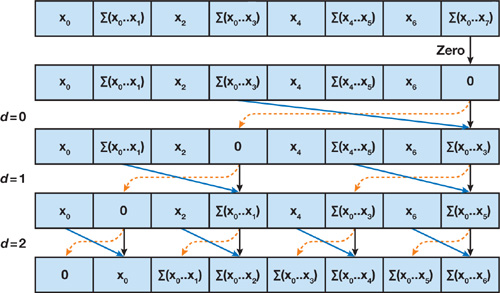
\includegraphics[width=\textwidth]{DownSweepScan.jpg}
    \caption{Down-sweep phase of parallel sum scan. Reproduced from\cite{nguyen2007gpu}}
    \label{fig:downsweepscan}
\end{figure}
\section{Stream Compaction}
In parallel computing, stream compaction is a useful tool for selecting a subset of data and compressing it into a coherent memory block. For example, stream compaction could be used to transfer all of the odd elements in array A of Figure~\ref{fig:streamcompactexample} and place them in order compressed at the start of array B.

\begin{figure}[!htpb]
    \centering
    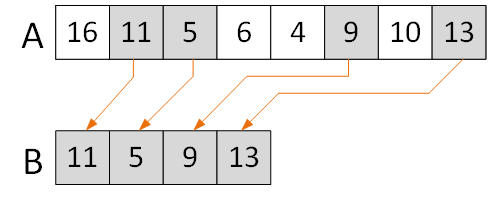
\includegraphics[width=0.8\textwidth]{StreamCompactExample.png}
    \caption{Example of stream compacting odd valued integers}
    \label{fig:streamcompactexample}
\end{figure}

Accomplishing this is surprisingly simple. As shown in Figure~\ref{fig:streamcompact}, a secondary array of flags is created. This array has a 1 for every odd number in array A and 0 for all others. An exclusive scan is performed on the flag array. Notice that every flagged element now has a unique zero-based index associated with it. The flagged elements are then ``scattered'' by the computed index. The scatter function is outlined in Algorithm~\ref{alg:scatter}.

\begin{figure}[!htpb]
    \centering
    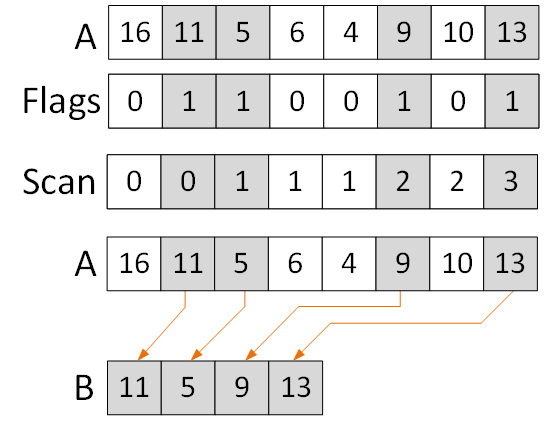
\includegraphics[width=0.8\textwidth]{StreamCompact.png}
    \caption{How stream compaction works (Scan and Scatter)}
    \label{fig:streamcompact}
\end{figure}


\begin{algorithm}[!htpb]
\label{alg:scatter}
 \singlespacing
 \KwData{input array A and scanned flag array F, both of length n}
 \KwResult{output stream compacted array B}
 \ForEach{i=0...n-1 in parallel}{
	\If{isFlagged(A[i])}{
 		B[F[i]] = A[i]\;
  	}
 }
 \caption{Sequential Sum}
\end{algorithm}

\section{Programming with CUDA}
CUDA is a C/C++ based programming language created by NVIDIA to expose the general compute functionality of their GPU processors. 
\subsection{CUDA GPU Architecture}
CUDA divides the computer into host and device. The host refers to the CPU and all memory it has access to, and the device refers to the GPU and its memory banks. Memory transfers between the host and GPU are started and managed by the host.\par
A piece of code that runs in parallel on the device is called a kernel. Figure~\ref{fig:kernelorganization} shows how kernels are organized. Each individual running process is called a ``thread''. Threads are organized into ``blocks'' of up to 1024 threads on modern architectures. Blocks are then grouped into ``grids''. Within each block, threads are executed in groups of 32 threads called ``warps''. Every thread in a single warp executes simultaneously on a single processor core.
The device memory architecture is depicted in Figure~\ref{fig:cudamemoryorganization}. Global memory, constant memory, and texture memory are all accessible by any thread in the kernel. Every thread also has access to a limited amount of memory which is shared between all threads in a block. Shared memory is much faster than global memory access, and can be used to accelerate kernels that need to share data between threads locally. Finally each thread has access to its own local register memory.

\begin{figure}[!htpb]
    \centering
    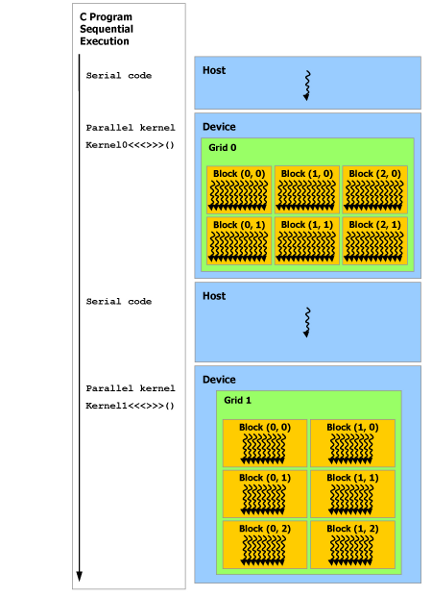
\includegraphics[width=1.0\textwidth]{CUDAKernelModel.png}
    \caption{CUDA Kernel Organization. Reproduced from \cite{cudadocumentation}}
    \label{fig:kernelorganization}
\end{figure}

\begin{figure}[!htpb]
    \centering
    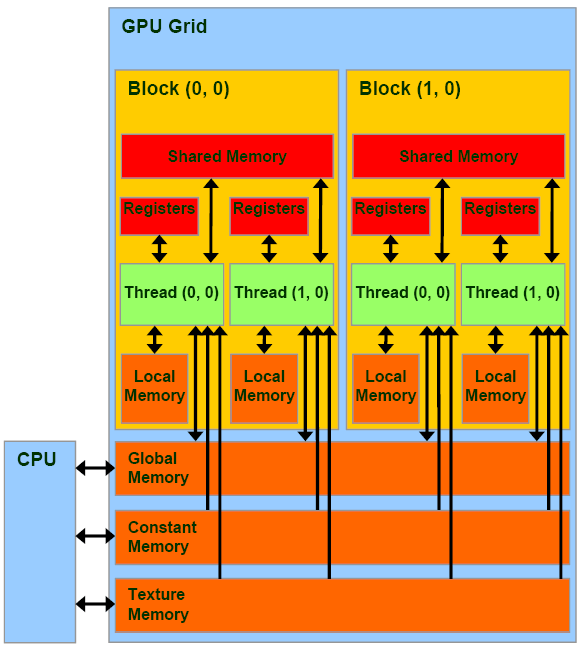
\includegraphics[width=1.0\textwidth]{CUDAMemoryModel.png}
    \caption{CUDA Memory Organization. Reproduced from \cite{gep3d}}
    \label{fig:cudamemoryorganization}
\end{figure}

\subsection{Optimizing CUDA Code}
Optimizing CUDA kernels is very application dependent and difficult to provide a universal manual for. However, there are several key underlying GPU architecture features that should be highlighted which can have a dramatic impact on performance.
\paragraph{Global Memory Coalesced Access} Global memory is designed in such a way that each half warp can load 64 consecutive bytes in memory as a single parallel read, provided the memory chunk is also 64-byte aligned. This is just enough memory to load an array of 16 consecutively floats at once (one per thread per half warp). To achieve peak memory bandwidth, reads and writes from global DRAM should be grouped into large consecutive chunks of memory. Because of this, it is sometimes extremely beneficial to utilized structure of array (SoA) data storage schemes as opposed to the more typical array of structures model (AoS).
\paragraph{Shared Memory Optimization}
Shared memory is much faster than global memory, so it can be instrumental in optimizing kernels. For example, instead of performing a reduction or scan in global memory, the entire array can be loaded into shared memory in a single read operation. The operation would then be performed in shared memory and the results written back in a single coalesced DRAM write. However, shared memory is limited. If too much is used, the number of blocks that can be simultaneously executed on a multiprocessor could go down, preventing the kernel from fully utilizing the GPU hardware. Also, this provides motivation for restricting the size of input data. If all of the data to be processed can be loaded into a single block, shared memory becomes much easier to utilize.\par
Shared memory is divided into banks, where successive 32-bit words are assigned to successive banks. Shared memory access is done per bank, so if every thread in a warp reads from a different bank, regardless of the ordering, no bank conflicts occur. If two or more threads try to read from the same bank simultaneously, the reads are serialized which reduced the shared memory bandwidth utilization. The exception to this rule is when all threads read from the same bank. This triggers a special broadcast mode that has no bandwidth penalty.
\paragraph{Warp Partitioning and Divergent Code}
As mentioned above, threads are actually executed in groups of 32 threads called warps. All threads in a warp take the same amount of time to operate. So if only one thread in a warp is actually doing any work, 31 threads will be idle and waste GPU hardware. Minimizing intra-warp code divergence in will go a long way towards fully utilizing hardware. Also, if possible retire entire warps early to free up resources for warps in the execution queue.